This chapter explores the effects of the resolution limit on the study of real brain connectivity networks.
We demonstrate that the resolution limit prevents detection of important details of the brain modular structure, thus hampering the ability to appreciate differences between networks and to assess the topological roles of nodes.
We show that Surprise in binary networks and Asymptotical Surprise in weighted networks do not suffer from these limitations.
Surprise maximization in brain co-activation and functional connectivity resting state networks reveals the presence of a rich structure of heterogeneously distributed modules, and differences in networks' partitions that are undetectable by resolution-limited methods. Moreover, Surprise leads to a more accurate identification of the network's connector hubs, the elements that integrate the brain modules into a cohesive structure.


\section{Surprise optimization on functional connectivity networks}\label{sec:surprise_optimization_fc_networks}
We assessed the performance of Surprise maximization by means of FAGSO in the detection of the community structure of two benchmark brain networks. All coordinate data and functional metadata were taken from the BrainMap database~\cite{fox2002,laird2005}, processed by Crossley et al.~\cite{crossley2013a} and made available to the scientific community as reference networks through the public Brain Connectivity Toolbox~\cite{rubinov2010}. We used BrainNetViewer as a tool for the visualization of the communities on brain templates~\cite{xia2013}.

\subsection{Resting state dataset}
The first network represents the coactivation of brain regions as obtained from a meta-analysis of 1641 task-related fMRI or PET studies~\cite{crossley2013a}.
Meta-analyses have been useful in estimating the frequency with which two brain regions are consistently activated across different tasks and are an indication of the behavior of the brain during activity.
Jaccard similarity, i.e. the number of studies activating both regions divided by the number of studies activating either one of them, was used as index to evaluate strength of the coactivation of 638 parcellated brain regions. More details on the construction of the network are available in~\cite{crossley2013a}.

The second network that we considered is a resting state functional connectivity network obtained from correlations between time series of fMRI signals, from a group study of 27 healthy subjects. In short, fMRI data were acquired from 27 healthy volunteers at 3T. Gradient echo-planar imaging data were collected for 5 min with 2s TR and 13 and 31 ms echo-times. Thirty six interleaved 3mm slices with in-plane resolution of $3.5\times 3.5$ mm were acquired. 
Time series were extracted from 638 brain regions defined by a template~\cite{crossley2013a}, corrected for motion and band-passed (0.01–0.1Hz).
Functional connectivity was defined in terms of pairwise Pearson correlations at a subject's level.
A group-level functional connectivity matrix was calculated by averaging individuals' matrices after Fisher-transform\footnote{A mathematical transformation needed to correctly compute averages of correlation coefficients. Fisher transformation of a correlation coefficient $-1 \leq r \leq 1$ is computed as $\tanh(r)$ and ranges from $-\infty$ to $+\infty$.}, and thresholded to retain 18625 edges, as described in Crossley et al.~\cite{crossley2013a}.
Ethical statements are present in the original references by the groups who performed the experiments. 
The resting state network was built using the same set of 638 regions and thresholded to have the same number of edges as in the coactivation study.
Both networks have been previously studied using Modularity-based algorithms and node-classification methods~\cite{crossley2013a}.

Due to its definition in terms of binomial coefficients, Surprise can be computed for integer values of its parameters.
We have therefore binarized the two adjacency matrices retaining an equal number of edges for both networks.
While the binarization process discards information contained in the edge weights, a judicious choice of threshold can ensure robust decomposition of the network~\cite{meunier2010,he2009}.
We have checked this statement by percolation analysis, a natural and non-arbitrary method to derive binary graphs from continuous adjacency matrices (see section~\ref{sec:percolation_analysis}).
Specifically, we have studied the size of the largest connected component of the coactivation and resting state networks removing iteratively the smallest weight edges.

This analysis, shown in Figure~\ref{fig:figure_8_percolation_analysis}, revealed the presence of percolation-like transitions, whereby the largest component of the network drops in jumps with increasing binarization threshold. For the coactivation and the resting state networks we found that the thresholds adopted by~\cite{crossley2013a} of 0.015576 and 0.600, respectively, are above the first jump in the size of the largest connected components and maintain network connectedness while ensuring that the networks are sufficiently sparse and possess the same number of edges. Hence, we adopted these thresholds for network's binarization. Analysis of the structures of networks obtained by a range of thresholds around these values showed stable solutions, with Normalized Mutual Information close between partitions close to 1, and a stable number of communities (Figures~\ref{fig:figure_9_rs_threshold_study} and \ref{fig:figure_10_rs_threshold_study}).

\begin{figure}[htb!]
\centering
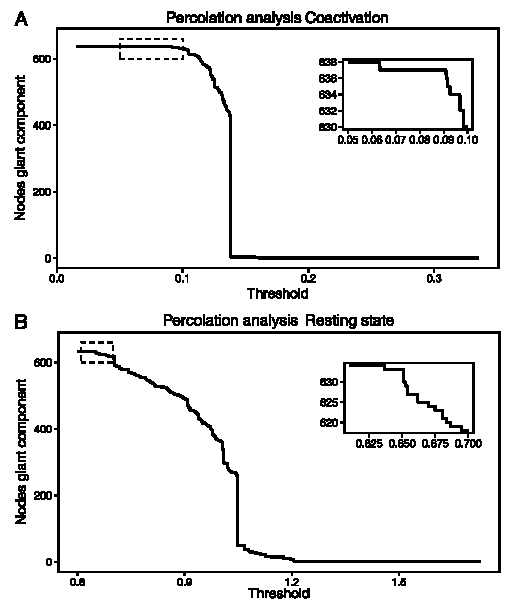
\includegraphics[width=0.7\linewidth]{images/figure_8_percolation_analysis_compressed.pdf}
\caption{Percolation analysis for the coactivation matrix (A) and resting state matrix (B).}
\label{fig:figure_8_percolation_analysis}
\end{figure}

\begin{figure}[htb!]
\centering
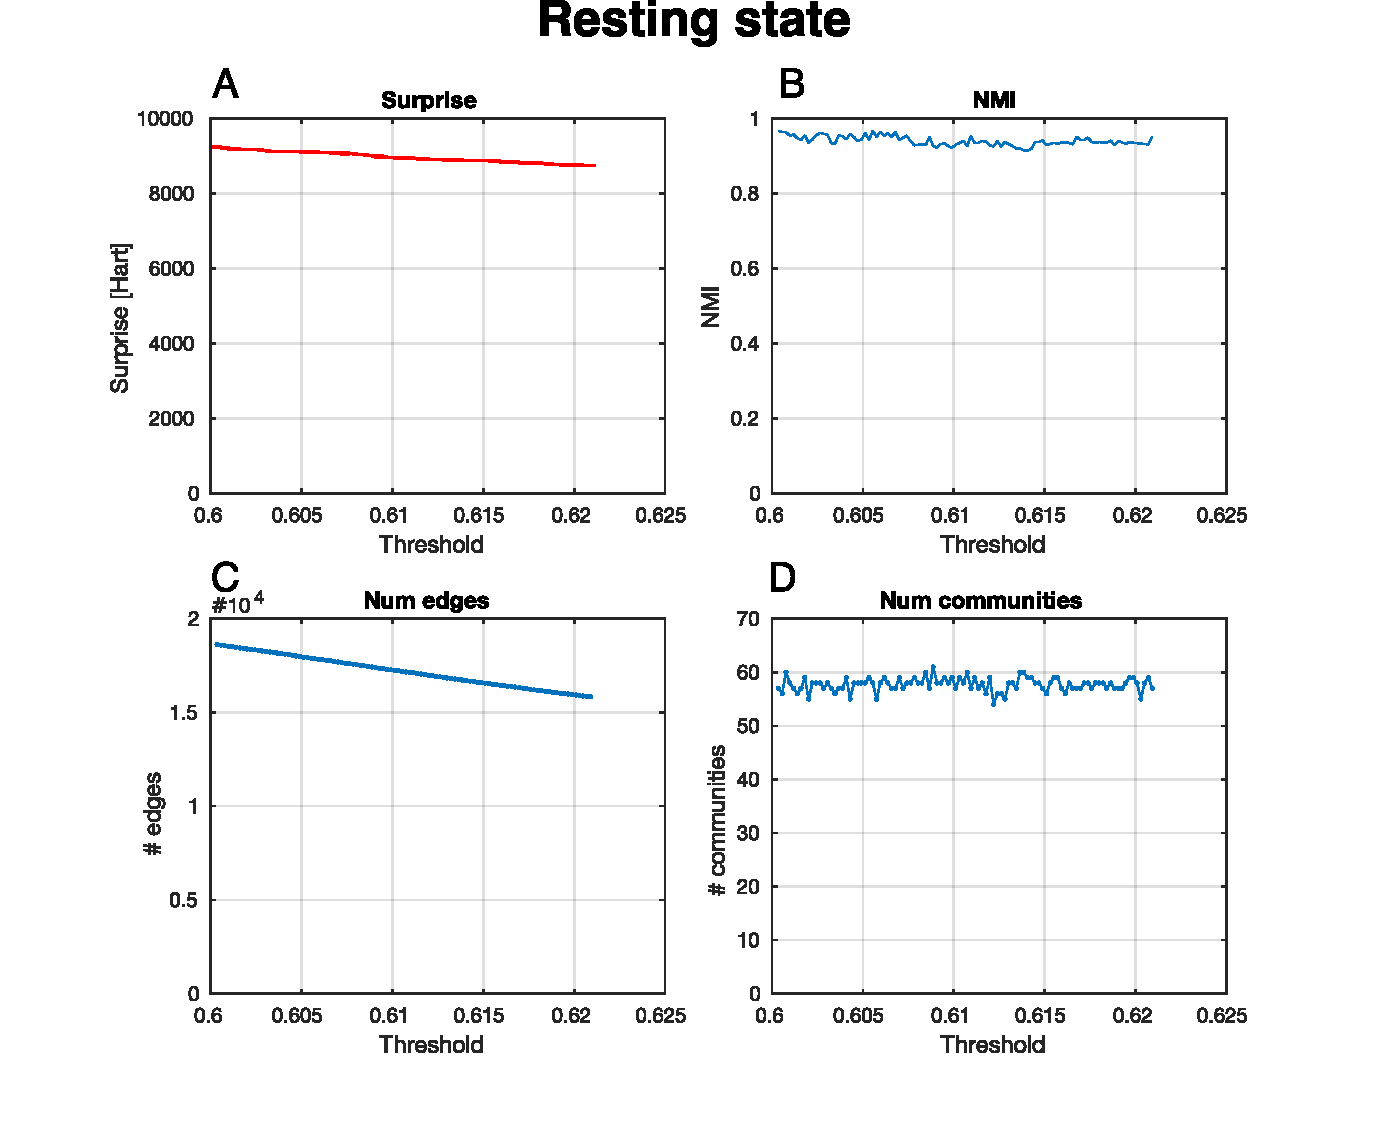
\includegraphics[width=0.7\linewidth]{images/resting_state_study_threshold.pdf}
\caption{Different Resting State networks were generated varying the binarization threshold in a range that changed the number of edges up to the 15th quantile of the edge weight distribution. This corresponds to threshold ranges of 0.015-0.03 for the co-activation network, and 0.60-0.62 for the resting state network. The resulting networks were partitioned by Susrprise maximization. The value of Surprise, the Normalized Mutual Information between the resulting optimal partitions, the number of edges and the number of communities are reported in panel A, B, C and D, respectively.}
\label{fig:figure_9_rs_threshold_study}
\end{figure}

\begin{figure}[htb!]
\centering
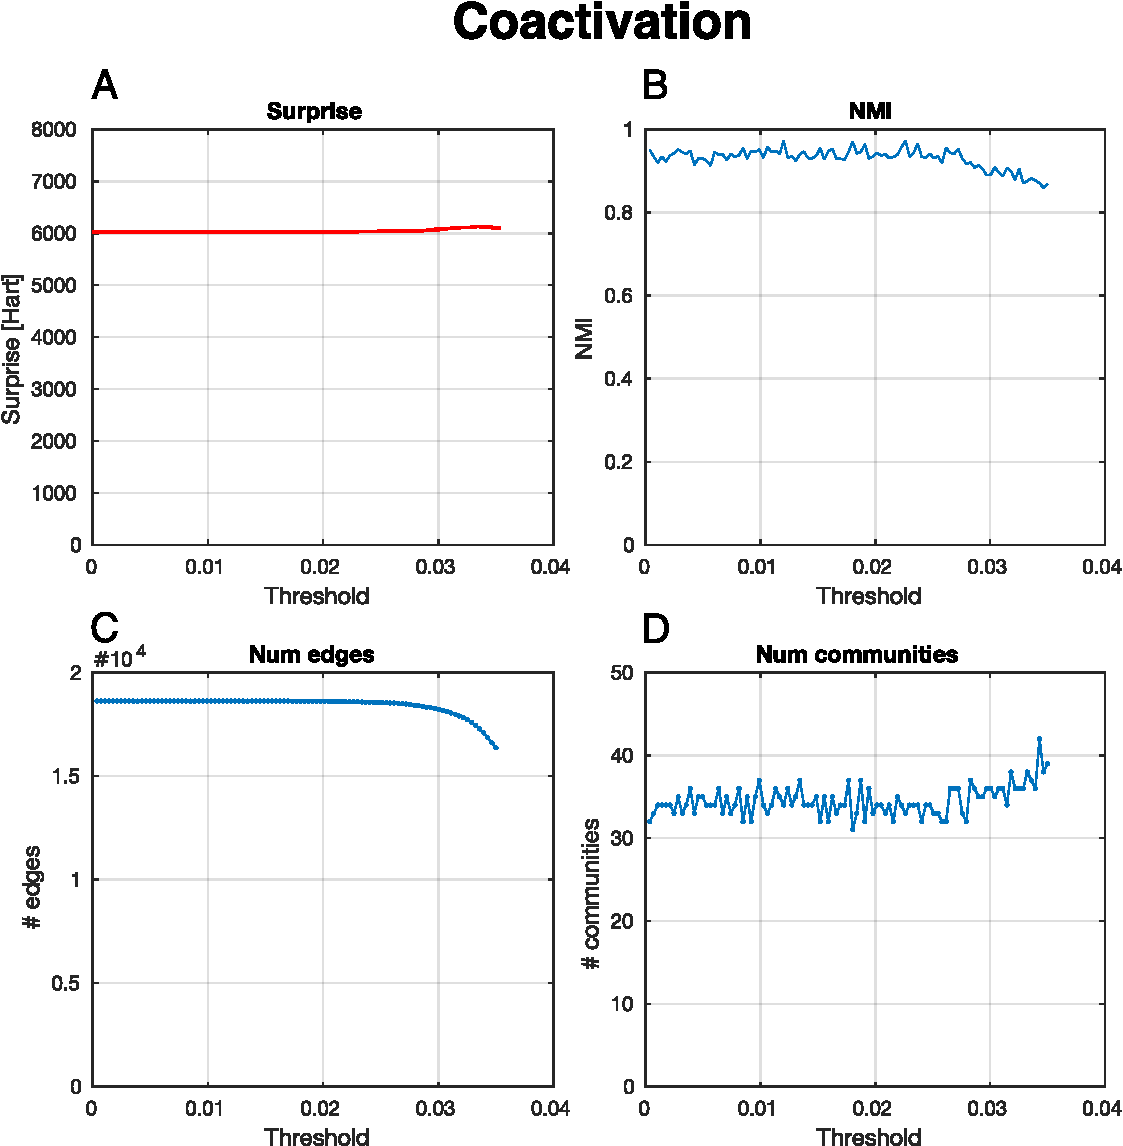
\includegraphics[width=0.7\linewidth]{images/coactivation_study_threshold.pdf}
\caption{Different coactivation networks were generated varying the binarization threshold in a range that changed the number of edges up to the 15th quantile of the edge weight distribution. This corresponds to threshold ranges of 0.015-0.03 for the co-activation network, and 0.60-62 for the resting state network. The resulting networks were partitioned by Susrprise maximization. The value of Surprise, the Normalized Mutual Information between the resulting optimal partitions, the number of edges and the number of communities are reported in panel A, B, C and D, respectively.}
\label{fig:figure_10_rs_threshold_study}
\end{figure}

\subsection{Community detection results by FAGSO}
Figure \ref{fig:figure_3_communities_rs_coact_mod_surp} shows a direct comparison of the partitions obtained by Modularity and by Surprise maximization for the coactivation and resting state networks. The four panels display the adjacency matrices of the two networks, with their vertices rearranged by their module membership.

\begin{figure}[htb!]
\centering
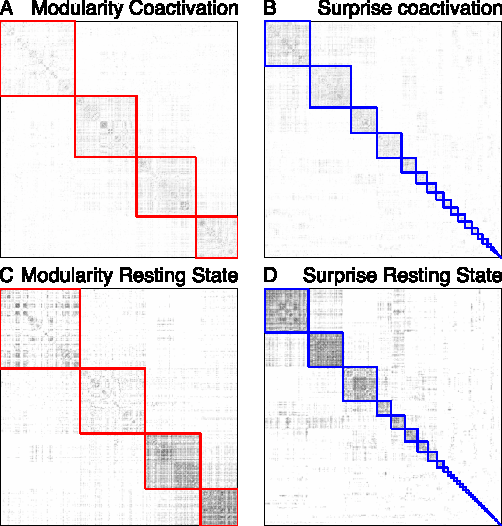
\includegraphics[width=1\linewidth]{images/figure_3_communities_rs_coact_mod_surp.pdf}
\caption{Modular structure of the coactivation and resting state networks under Modularity and Surprise maximization. The node indexes have been reordered by membership to highlight the modules, which are demarcated by a red line, for Modularity, or a blue line, for Surprise. Modularity maximization identifies only four, large modules, consistent with previous analysis of these data-sets. Surprise reveals a much finer and complex modular structure.}
\label{fig:figure_3_communities_rs_coact_mod_surp}
\end{figure}

By Newman’s decomposition, the resting state and coactivation brain networks present a modular structure with four large modules that have been anatomically labeled as occipital, central, frontoparietal and Default Mode networks~\cite{crossley2013a} (demarcated by a red line in Figure \ref{fig:figure_3_communities_rs_coact_mod_surp}). These partitions are highly similar (Rand Index 0.78), despite the different neurofunctional bases of the two networks~\cite{smith2009} and comprise modules that are relatively uniform in terms of number of nodes and number of edges within each module.

The partitions obtained by Surprise maximization for the two networks are shown in Figure \ref{fig:figure_3_communities_rs_coact_mod_surp}B, \ref{fig:figure_3_communities_rs_coact_mod_surp}D. Surprise found 51 communities, $\hat{S}=8969.24$, for the resting state network, and 28 communities, $\hat{S}=5725.65$ for the coactivation network.
These modules are delimited by blue lines that show the wide distribution in size of the components, ranging from communities with 119 nodes and 4586 edges down to singletons.
The size distributions of the modules are different for the two networks, with a more rapid drop and a fatter tail in the coactivation network compared with the resting state network.

The complete list of communities, with anatomical labels and stereotaxic coordinates for all nodes~\cite{laird2010,lancaster2007,tzourio2002}, as well as the density and number of nodes of each community found by Modularity and Surprise optimization, are reported in tabular form in the appendix (Tables~\ref{tab:densities_tables_mod_coact},~\ref{tab:densities_tables_modularity_rs},~\ref{tab:densities_tables_surprise_coact},~\ref{tab:densities_tables_surprise_rs}).

Analysis by Surprise suggests that the modular structure of resting state functional connectivity brain networks comprises modules of very different sizes, in sharp contrast with previous studies that have used resolution-limited functions like Newman's Modularity (see~\cite{meunier2010} for a review).
To emphasize this point, we have also partitioned the coactivation and resting state networks using Infomap~\cite{rosvall2008} and a multiscale version of Modularity with an adjustable resolution parameter~\cite{reichardt2006} provided by the Brain Connectivity Toolbox~\cite{rubinov2010}.
Interestingly, increasing the resolution parameter results in a larger number of smaller communities that are however characterized by a relatively homogenous size distribution, a result of the intrinsic scale built into these methods (Figure~\ref{fig:figure_11_gamma_1_75_rs_coact}).
Additionally, we have made a quantitative comparison between the partitions obtained by Surprise, Infomap and the Reichardt and Bornholdt's method~\cite{reichardt2006} by calculating the Normalized Mutual Information between the resulting community structures (Tables~\ref{tab:coact_nmi_fagso}~\ref{tab:rs_nmi_fagso}). Despite the fact that these methods retrieve a few more modules that Newman's Modularity, they fail to capture the heterogeneous distribution of clusters revealed by Surprise. 

In order to assess the significance in neurofunctional terms of the finer partitions obtained by Surprise, we show the node distribution as an overlay of the MNI brain atlas template for the 10 largest modules of the resting state network in Figure \ref{fig:figure_4_resting_state_communities}. The communities highlighted by Surprise show a correspondence with some well-known functional networks previously identified by multivariate analysis (e.g. Independent Component Analysis) of functional MRI data~\cite{raichle2001,salvador2005,damoiseaux2006,deluca2006}, and with well-defined, segregated anatomical or functional districts.

\begin{figure}[htb!]
\centering
\includegraphics[width=1\linewidth]{images/figure_4_resting_state_communities.pdf}
\caption{The ten largest modules found by Surprise in the resting state network overlaid on an MRI brain template. The module indexes are ordered by decreasing size. The modules are named after corresponding functional networks previously identified by multivariate analysis of resting state fMRI data.}
\label{fig:figure_4_resting_state_communities}
\end{figure}

\begin{figure}[htb!]
\centering
\includegraphics[width=1\linewidth]{images/figure_5_communities_comparison.pdf}
\caption{Comparison of selected modules in the partition obtained by Surprise in the resting state and coactivation networks. The indexes are inversely ranked according to the size of the modules in their respective networks.}
\label{fig:figure_5_communities_comparison}
\end{figure}

\begin{figure}[htb!]
\centering
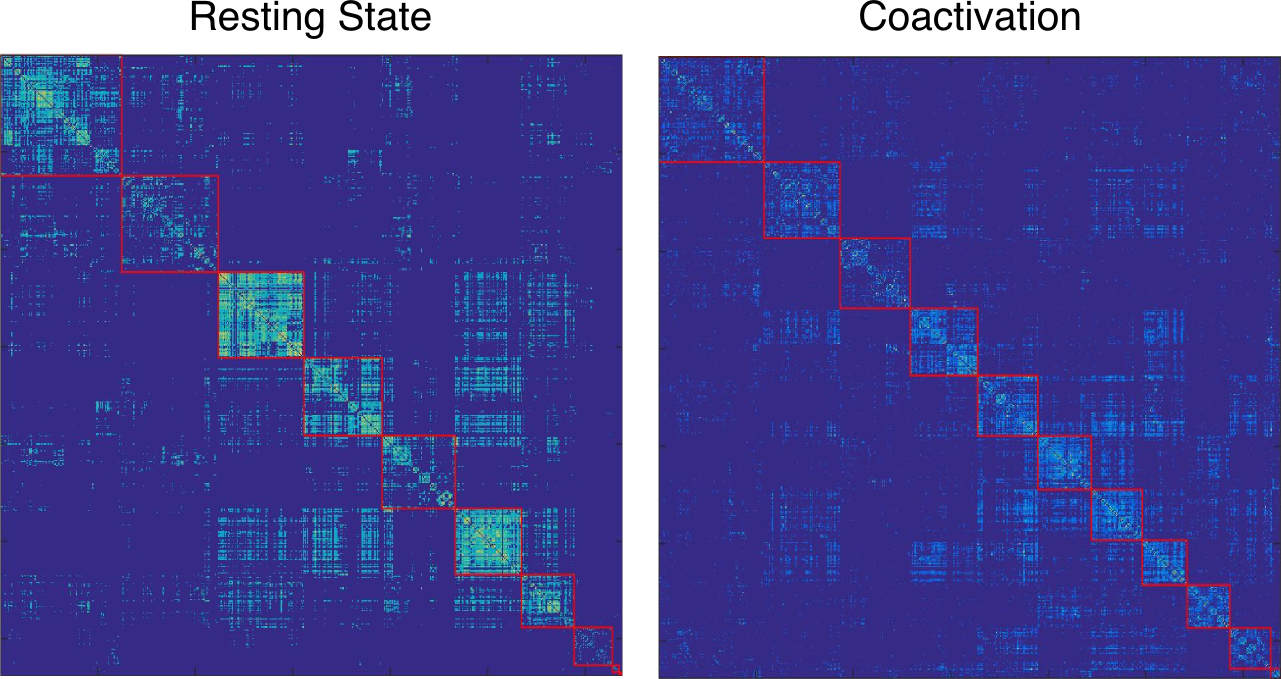
\includegraphics[width=1\linewidth]{images/coact_rs_gamma_1_75.png}
\caption{Partitions obtained with multiresolution Modularity (Reichardt and Bornholdt method) for a value of the resolution parameter $\gamma=1.75$ for the coactivation and resting state networks. Increasing the resolution parameter improves detection of smaller modules, but breaks up larger ones, thus resulting in relatively homogeneous size distributions.}
\label{fig:figure_11_gamma_1_75_rs_coact}
\end{figure}

\begin{table}
\centering
\begin{tabular}{ccccc}
& & \textbf{Coactivation} & \\
\hline 
\textbf{NMI} &Modularity & Surprise & Infomap & RB $\gamma=1.75$ \\
\hline
Modularity 			& \textbf{1.00} & 0.61 & 0.56 & 0.61 \\
Surprise 			& 0.61 & \textbf{1.00} & 0.54 & 0.62 \\
Infomap 			& 0.56 & 0.54 & \textbf{1.00} & 0.59 \\
RB $\gamma=1.75$ 	& 0.59 & 0.61 & 0.59 & \textbf{1.00} \\ \hline 
\end{tabular}
\caption{Normalized Mutual Information between partitions of the coactivation network with Newman's Modularity, Infomap, Reichardt and Bornholdt and Surprise.
We used the Fagso algorithm for Surprise maximization, the \texttt{igraph} implementation of Infomap, the Brain Connectivity Toolbox implementation for RB (\texttt{community\_louvain.m} function) and \texttt{modularity\_und.m} for Modularity.
For each method the best solution over 100 repetitions was used to calculate NMI.}
\end{table}

\begin{table}
\centering
\begin{tabular}{ccccc}
& & \textbf{Resting State} & \\
\hline 
\textbf{NMI} &Modularity & Surprise & Infomap & RB $\gamma=1.75$ \\
\hline
Modularity & \textbf{1.00} & 0.52 &  0.70 & 0.66 \\
Surprise & 0.52 & \textbf{1.00} & 0.53 & 0.58 \\
Infomap & 0.70 & 0.53 & \textbf{1.00} & 0.68 \\
RB $\gamma=1.75$ & 0.66 & 0.58 & 0.68 & \textbf{1.00} \\ \hline 
\end{tabular}
\caption{Normalized Mutual Information between partitions of the Resting state network with Newman's Modularity, Infomap, Reichardt and Bornholdt and Surprise.
We used the Fagso algorithm for Surprise maximization, the \texttt{igraph} implementation of Infomap, the Brain Connectivity Toolbox implementation for RB (\texttt{community\_louvain.m} function) and \texttt{modularity\_und.m} for Modularity.
For each method the best solution over 100 repetitions was used to calculate NMI.}
\end{table}

\begin{table}
\centering
\begin{tabular}{lccccc}
& &\textbf{Coactivation}	&	&	&\\
\hline
&\textbf{NMI}&	Surprise &	Infomap&	RB $\gamma=1.75$\\ \hline
\textbf{RS} &Surprise& 0.59&0.40&0.52\\
	&Infomap & 0.54&0.44&0.51\\
	&RB $\gamma=1.75$ &0.59&0.41&0.53\\ \hline 
\end{tabular}
\caption{Normalized Mutual Information between Resting State (RS) and Coactivation (Coact) partitions. Infomap and RB methods are repeated 100 times and partitions with the highest quality are used. NMIs are approximated to second significant digit.}
\end{table}

The largest communities of the resting state network correspond to the primary sensorimotor cortex~\cite{biswal1995}, primary visual and extra-striate visual network, fronto-parietal lateralized networks~\cite{smith2009} as well as the so-called default mode network (DMN)~\cite{raichle2001,fransson2006}.
The attentional frontoparietal networks (FPAN)~\cite{beckmann2005} were detected as two separate, lateralized subnetworks, in agreement with~\cite{deluca2006} although other studies have identified a single, bilateral FPAN~\cite{markett2014}.

Smaller networks, like the executive control and auditory networks~\cite{salvador2005,vandenheuvel2010} were also resolved by Surprise, as well as subcortical structures, like the hippocampal and thalamic formations~\cite{roy2009,chen2013}. Interestingly, the thalamic nuclei appear as one tight community, despite the fact that they are structurally unconnected, in keeping with the idea that functional connectivity does not necessarily require the presence of strong structural links.

The more accurate partition afforded by Surprise may enable identification of differences in the modular structures of networks that cannot be appreciated with a resolution limited method. By way of example, we have compared the partitions of the resting state and coactivation networks (Figure \ref{fig:figure_5_communities_comparison}). Indeed, these networks are of a different nature, the former representing intrasubject baseline fluctuations in the brain's resting state, and the latter the responses to a variety of different tasks across subjects. However, Newman's Modularity finds similar partitions for these two networks, with 4 large modules each.

Conversely, under Surprise maximization, the partition of the resting state network shows many more small communities comprising less than 5 nodes (32 in total) compared with the coactivation one (only 11). Moreover, certain communities of the resting state network appeared to be split into smaller modules in the coactivation matrix. 
By way of example, the cuneus and the lingual and pericalcarine gyri were part of the occipital visual module in the resting state, but not in the coactivation network, where they formed a separate community (first row of Figure \ref{fig:figure_5_communities_comparison}).
Similarly, the precuneus and medial parts of the postcentral girus were identified as an independent community in the coactivation network, while they were part of the broad somatosensory network in the resting state connectivity graph~\cite{rubinov2011} (second row of Figure \ref{fig:figure_5_communities_comparison}).
Interestingly, the Broca area, indicated as Module 11 in Figure \ref{fig:figure_5_communities_comparison}, was separated from the auditory network in the coactivation network, and identified as a small, but anatomically and functionally distinct, community.
Conversely, other communities were split in the resting state but not in the coactivation network. The executive and attentional control networks were merged into a large community in the coactivation network, while they were separated under resting state conditions, including a subdivision of the left and right fronto-parietal networks (third row of Figure \ref{fig:figure_5_communities_comparison}).

While the resting state and coactivation networks appeared to possess virtually identical modular structures under Newman's analysis, they showed functionally and anatomically relevant differences when analyzed by Surprise maximization, with a Normalized Mutual Information between the partitions of the two networks of 0.5922. Indeed, Modularity tends to assign small communities to larger structures even when they correspond to tightly-knit modules, thus concealing differences in the graphs' modular structures that involve aggregation or disaggregation of smaller clusters. It is conceivable that the detrimental effects arising from the resolution limit may have affected previous studies comparing different populations~\cite{meunier2010}.
Surprise may offer a sharper tool to detect alterations of brain connectivity induced, for example, by psychiatric or neurological conditions, thus enabling the exploration of novel markers of brain disease.

\subsection{Hubs classification}
Besides the exploration of functional and anatomical segregation, understanding the modular structure of brain networks is critical for the interpretation and classification of the roles played by the nodes within the network structure~\cite{sporns2007}. Highly connected nodes, or hub nodes, are particularly important for their topological centrality, and function as integrators. Hubs that primarily connect to nodes within the same module are dubbed ``provincial hubs'', and nodes that connect different modules are referred to as ``connector hubs''. The former are thought to be responsible for the formation and stability of the modules, while the latter ensure integration of the activity of the different modules. Obviously, interpretation of the hub's role relies on the correct identification of the optimal network partition, and may be strongly affected by the resolution limit.

Here, we have performed a hub's role analysis for the resting state and coactivation networks under Modularity and Surprise maximization.
To this end, we have adopted Guimera' and Amaral classification scheme~\cite{guimera2005}, whereby nodes are classified by their within-community degree $z$ (a measure of how well-connected a node is to other nodes in the same community) and their participation coefficient $P$, a parameter that is $0$ for nodes with purely intra-module connections and $1$ for nodes whose links project primarily to other modules. 

Figures \ref{fig:figure_6_ga_rs_coact}A and \ref{fig:figure_6_ga_rs_coact}B show the different positioning of high-degree nodes in the Guimera' and Amaral plot for the coactivation and resting state networks partitioned using Newman’s approach and Surprise maximization. In this scheme, provincial hubs are high-degree nodes that score high $z$ and low $P$ values (\emph{R5} region); conversely, connector hubs are characterized by larger $P$ values (regions on the right-hand side of the plot).

\begin{figure}[ht!]
\centering
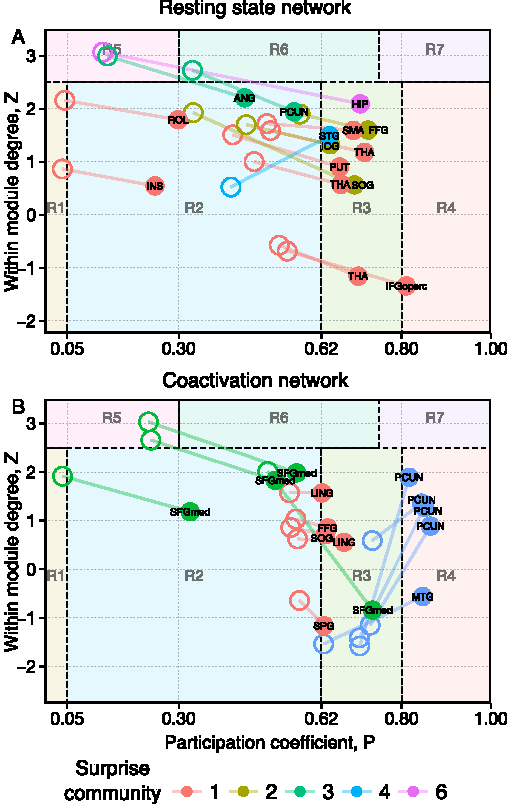
\includegraphics[width=0.5\linewidth]{images/figure_6_ga_rs_coact.pdf}
\caption{Classification of representative nodes according to their intra- and intermodule connections for the resting state (A) and coactivation (B) networks. Empty circles and full circles indicate the position of each node in the Guimera' and Amaral’s plot after partition by Modularity or Surprise, respectively. An overall increase in the participation coefficient, a measure of the intermodule connectivity, is observed for the Surprise partition relative to the Modularity partition. To avoid cluttering of the graph, we only reported those nodes with a degree higher than the average within a Standard Deviation, and whose classification is different in the two partitions. The abbreviations of the brain regions corresponding to the nodes are reported in the appendix, Table~\ref{tab:abbreviations}.}
\label{fig:figure_6_ga_rs_coact}
\end{figure}

A finer partition in smaller communities may be expected to determine an overall increase in participation coefficient and decrease in within-community degree. However, the heterogeneous partitions obtained by Surprise maximization resulted in non-trivial changes in the Guimera' and Amaral classification. By way of example, we discuss in greater detail two regions whose roles are very different in the two partitions, to highlight the effects of the resolution limit.

Nodes that belong in the hippocampal formation show a large within-module coefficient, and appear as provincial hubs (region R5 of Figure \ref{fig:figure_6_ga_rs_coact}) under Modularity optimization. However, their participation coefficient increases 6-fold in the partition by Surprise, which reveals a role as connectors for these nodes, with widespread projections to many other modules across the brain, including the module 3, 6, 8, 5, 2, corresponding to the DMN, the amygdala and parahippocampal formation, the temporal inferior gyrus, the cuneus and lingual gyrus, and the visual cortex, respectively.
This finding is in agreement with the idea that the hippocampus acts as ``network convergence zone'', as it receives polysensory input from distributed association areas in the neocortex~\cite{misic2014}.

Interestingly, the right shift in the Guimera-Amaral plot is less pronounced for the nodes in the posterior part of the hippocampus (Figure \ref{fig:figure_7_ga_coact_hippocampus}). A differential classification of the anterior and posterior hippocampus is consistent with the hypothesis of a functional differentiation of this structure~\cite{moser1998}, with the posterior hippocampus mostly involved in memory and cognition, and the anterior hippocampus playing a role in the processing of stress, emotion and affect~\cite{fanselow2010}. Moreover, studies in animal models have shown differential organization of the efferent connections of the hippocampal formation~\cite{swanson1977}, consistent with different functions for the anterior and posterior hippocampus.

\begin{figure}[htb!]
\centering
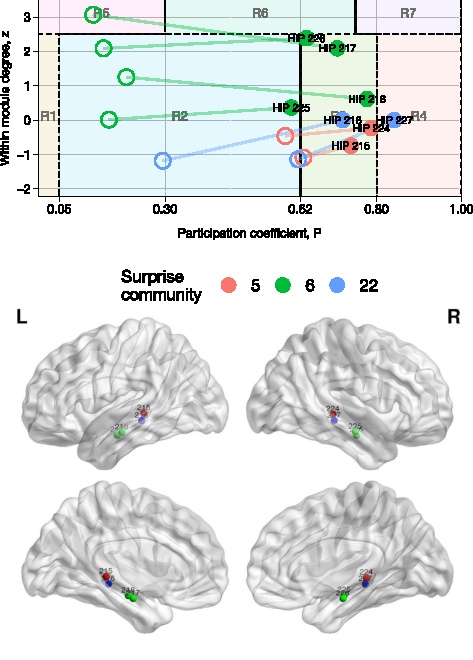
\includegraphics[width=0.5\linewidth]{images/figure_7_hippocampus.pdf}
\caption{Top panel: classification of all the hippocampal nodes according to the Guimera' and Amaral's scheme for the coactivation network. Empty circles and full circles indicate the position of each node after partition by Modularity or Surprise, respectively. Bottom panel: anatomical positions of the nodes in the hippocampal formation, colored by Surprise community membership. The increase in participation coefficient upon partition by Surprise is more pronounced for nodes in the anterior part of hippocampus, with an antero-posterior gradient.}
\label{fig:figure_7_ga_coact_hippocampus}
\end{figure}

Similar rightward shifts for nodes and hubs were observed in the resting state network, and reported in Figure \ref{fig:figure_6_ga_rs_coact}.
However, increases in participation coefficients are by no means the only differences in the classification of nodes obtained by Surprise maximization. A prominent example is the precuneus (PC) (Figure \ref{fig:figure_6_ga_rs_coact}B, blue dots) that shows a high participation coefficient in both partitions by Modularity and Surprise, but a much higher within-module degree under Surprise maximization.

Indeed, the nodes comprised in the precuneus intrinsically possess high inter-cluster connectivity, but are distributed among the four modules found by Modularity. In the partition by Surprise they are grouped together, and this precuneal module as a whole plays a connector's role integrating different communities (Figure \ref{fig:figure_8_ga_rs_precuneus}), a hypothesis that is consistent with the precuneus supporting a wide spectrum of highly integrated tasks, from visuo-spatial imagery to episodic memory retrieval and self-processing operations~\cite{cavanna2006}.

In summary, partition by Surprise maximization results in very different distributions of participation coefficients and within-module degree compared to Modularity. These differences are not uniform across nodes, and arise from the limited ability of Modularity to identify small modules. Finer partition by Surprise reveals very different roles for some key brain areas, and suggests that a systematic reanalysis of the topological roles of brain nodes and hubs may be in order.

\begin{figure}[htb!]
\centering
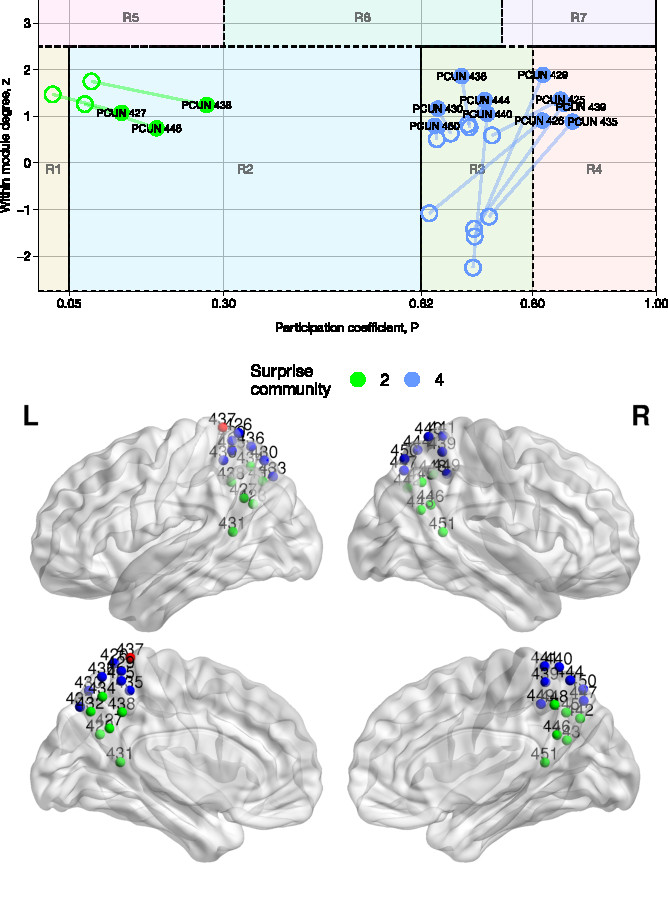
\includegraphics[width=0.5\linewidth]{images/figure_8_precuneus.pdf}
\caption{Top panel: classification of the precuneal nodes according to the Guimera' and Amaral's scheme for the resting state network. Empty circles and full circles indicate the position of each node after partition by Modularity or Surprise, respectively. Bottom panel: anatomical positions of the nodes in the precuneus, colored by Surprise community membership. The nodes in the dorsal part of the precuneus exhibit a sharp increase in within-module degree.}
\label{fig:figure_8_ga_rs_precuneus}
\end{figure}

\subsection{Limitations of binary Surprise}

A potential limitation of Surprise is related to its definition in terms of discrete probability distributions. This makes Surprise suited for the study of binarized networks. While the topological backbones of the networks we have investigated appear quite robust against removal of lowest-weight edges and binarization, as shown by our percolation and stability analyses (Figures~\ref{fig:figure_8_percolation_analysis},~\ref{fig:figure_9_rs_threshold_study},~\ref{fig:figure_10_rs_threshold_study}), the application of its weighted counterpart, Asymptotical Surprise, will help overcome the need of binarization.

The superior resolution afforded by Surprise may make it more vulnerable than other methods to noise and experimental errors. Indeed, occasional misassignment of nodes due to noise-induced changes in edge distribution are likely to affect small modules, comprising only a few nodes, more than large ones. Hence, experimental uncertainty also limits resolution, and a resolution-limit-free method would not necessarily improve the quality of the partition in a scenario dominated by noise. 

To ascertain whether this is the case for the co-activation and resting state networks investigated here, we have simulated the effects of experimental errors by injecting noise into the distributions of weights prior to the binarization procedure, thus introducing variability in the connectivity structure of the resulting binary networks.
We set levels of noise sufficient to perturb up to 10\% of the edges of the final binary network. Using this procedure, for each level of noise we generated ten different graphs, and applied the Surprise Maximization algorithm to each of them. 

The ten different graphs were generated by adding noise to the off-diagonal elements of the adjacency matrix prior to the binarization procedure. The amplitude of noise was chosen to randomly perturb 10\% of the edges after binarization. Surprise maximization was applied to the resulting graphs. In the left panel of Figure~\ref{fig:figure_9_nmi}, we reported the Normalized Mutual Information (NMI) between the optimal partitions of each of the ten perturbed networks and that of the original resting state network.
The number of communities retrieved by FAGSO in each of the perturbed networks is reported in the right panel of Figure~\ref{fig:figure_9_nmi}. The graphs show that the partitions of the ``noisy'' graphs are consistent and similar to those of the unperturbed network, with NMI scores close to 1 and almost constant numbers of communities.
These results demonstrate that Surprise maximization can retrieve the network's community structure even in the presence of substantial noise in the data.
We found that the partitions of these graphs were highly consistent with those of the original networks (Figure~\ref{fig:figure_9_nmi}).

\begin{figure}[ht]
\centering
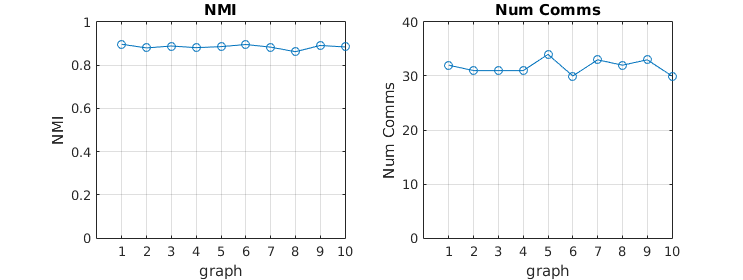
\includegraphics[width=1\linewidth]{images/figure_9_nmi.png}
\caption{Assessment of the effects of experimental error on the community structure of the resting state network.}
\label{fig:figure_9_nmi}
\end{figure}

We should also stress that there is no constraint in the FAGSO algorithm imposing inter-hemispherical symmetry of the partition.
Nevertheless, we observed homotopic correspondence in the community structure, and a close resemblance with established neurofunctional circuits as in Figure~\ref{fig:figure_4_resting_state_communities} and~\ref{fig:figure_5_communities_comparison}. Taken together, simulations of the effects of noise and qualitative considerations on the neurofunctional significance of the modules identified by Surprise corroborate the idea that experimental error is not the predominant factor in the networks investigated.

A final and important point we should highlight is that Surprise maximization, in the implementation we have used here, does not allow for overlapping communities. Other methods have been applied to investigate this aspect in brain networks~\cite{palla2005,ahn2010}. However, a recent comparative analysis of graph partitioning algorithms on a variety of benchmark networks~\cite{lancichinetti2009} has shown that these methods are also prone to merging overlapping communities, with relatively modest performance in recovering heterogeneous cluster distributions planted in model networks.
Despite these potential limitations, the resolution-limit-free behavior of Surprise makes it an excellent tool to explore and to overcome the effects of the resolution limit in the modular structure of brain connectivity networks.

% PARAGRAFO PER INCOLLARE I DISCORSI
\section{From binary to weighted functional connectivity}
The results obtained from binary Surprise optimization on real functional connectivity networks, encouraged us to extend the Surprise optimization approach to Asymptotical Surprise. Indeed, as the process of binarization irremediably looses the information carried by the edge weights, using Asymptotical Surprise would provide a new and important tool to study the modular organization of brain connectivity beyond the resolution limit.

Capitalizing on recent development in the field of statistical physics of complex networks~\cite{traag2015}, here we demonstrate the use of Asymptotical Surprise with the PACO optimization method, in the study of the modular structure of weighted networks.

Since there is no ground-truth structure for brain functional connectivity networks, we have assessed the performance of this novel approach on synthetic networks with a planted modular structure, and compared it to some of the leading graph partitioning methods, namely Louvain method for Newman's Modularity (see section~\ref{sec:louvain_method}) and Infomap.
Importantly, we demonstrate our approach in networks derived from synthetic data that mimic different structures, levels of noise and variability, such as those observed in functional connectivity experimental data.
Indeed, improved resolution afforded by Asymptotical Surprise may imply increased vulnerability to spurious modules resulting from noisy correlations.
It is therefore important to assess the benefits of increased resolution against the limitations arising from intrinsic data variability. 

Finally, we apply Asymptotical Surprise to weighted functional connectivity networks from resting state fMRI data, revealing a heterogeneous, multiscale community structure. We show that the finer modular subdivision of resting state functional connectivity networks obtained by Asymptotical Surprise leads to substantial differences in the identification of connector hubs compared to other community detection methods.

\subsection{Synthetic benchmark networks}
One important finding in~\cite{nicolini2016} is that brain networks are organized in modules with heterogeneous size distributions.
We implemented this property in our two types of benchmark networks.
For the first test, we generated a ring of cliques with $300$ nodes, and sizes of the cliques sampled from a power-law with exponent $\tau_c=2$, minimum and maximum clique size respectively $\min_c=5$, $\max_c=50$ (see also Supplementary Materials S4).
For each subject of the sample, we synthesized $150$ time-points for each node using the \texttt{neuRosim R} package~\cite{neurosim2011}.
We set the baseline value of all the time series to $100$~\cite{welvaert2013}.

Finally, we correlated the original synthetic time series $\mathbf{X}$ by multiplication with the matrix $\mathbf{L}$, obtained the correlated time series $\mathbf{Y}$ and added Rician noise~\cite{Gudbjartsson1995} to $\mathbf{Y}$ independently for each area. The simulated data $\mathbf{Y}$ did not include slow drift components, simulated physiological noise, nor spatial noise. The average SNR was defined as $\textsc{SNR}=\bar{S}/\sigma_N$ where $\bar{S}$ is the average magnitude of the signal and $\sigma_N$ is the standard deviation of the noise~\cite{kruger2011}.

In order to be more exhaustive and extend the validity of results, we repeated the same procedure on weighted LFR networks with $N=600$ nodes, sampling nodes degree from a power-law with exponent $\tau_d=2$, average degree $\left<k\right>=12$ and maximum degree $\max_k=50$.
We set the topological and weights mixing coefficients, i.e. the average fraction of intra-cluster and inter-cluster degree and strengths, to $\mu_t=0.1$ and $\mu_w=0.1$, respectively. Planted community sizes ranged from $5$ to $50$ nodes and were sampled from a power law with exponent $\tau_c=1$. In the Supplementary Information we have extended this analysis to a wider range of network parameters.

Group-level correlation matrices were computed by Fisher-transforming and averaging individual instances of the above matrices. Sparsification was obtained by removing edges with weights below the most stringent threshold that maintained the network connectedness, a procedure known as percolation analysis~\cite{gallos2012,bardella2016a,alexander-bloch2010}. This approach measures the size of the largest connected component of the network upon iterative removal of the weakest edges and enables data-driven determination of the optimal sparsification threshold that preserves network structure and connectedness while removing potentially spurious correlations.

The community structure of the resulting weighted sparsified matrices was detected by Asymptotical Surprise optimized with PACO and compared against two widely used methods, Infomap~\cite{rosvall2008} and Newman's Modularity~\cite{blondel2008,newman2006}, that are affected by the resolution limit, albeit to different extents. 
In Newman's Modularity, the size of the smallest detectable cluster is of the order of the square root of the number of edges in the entire network~\cite{fortunato2007}, while Infomap has a limit that depends on the overall number of inter-cluster edges~\cite{kawamoto2015}.
Here we used the Louvain implementation available in the Brain Connectivity toolbox~\cite{rubinov2010} and the Infomap implementation available in the \texttt{igraph-0.7.1} package~\cite{igraph2006}.

For all methods, including PACO, we launched $10,000$ independent runs, and picked the membership corresponding to the partition with the best value of the fitness function, the maximum for Modularity and Asymptotical Surprise, the minimum for Infomap.

As discussed in the previous chapter, sections~\ref{sec:degeneracy},~\ref{sec:degeneracy_surprise},~\ref{sec:degeneracy_asymptotical_surprise}, degeneracy of nearly-optimal solutions does not appear to severely affect Surprise or Asymptotical Surprise, and a consensus approach is not deemed necessary for these functions.
This analysis supports our choice to select the solution with the highest value of the fitness function.

\subsection{Measures of partition quality}
For each method, we analyzed the level of agreement of the detected community structure against the planted one in terms of Normalized Mutual Information (NMI)~\cite{danon2005}.
Additionally, we used two different coefficients of similarity between partitions: Sensitivity and Specificity. 

To this end, we quantified the confusion matrix $\mathbf{C}$ between the detected and planted modules. Each element $C_{ij}$ is the number of nodes in the planted community $i$ that appear in the detected community $j$.
For each planted community we scored as true positives (TP) the nodes correctly identified as belonging to the ground-truth community, and as false positives (FP) the nodes wrongly assigned to a community; similarly false negatives (FN) were nodes wrongly classified in different communities and true negatives (TN) the nodes correctly classified as out of the community.
Sensitivity, defined as $TP/(TP+FN)$, decreases with increasing number of False Negatives. Specificity instead is defined as $TN/(TN+FP)$ and decreases when many nodes are wrongly assigned in the same community.
Additionally, we computed Accuracy and Matthew Correlation Coefficient (see Supplementary Materials for definitions)\todo{mettere definizioni matthew correlation coefficient}.

% \subsection{Human resting state network}
% We applied Asymptotical Surprise maximization by PACO to the same reference resting state fMRI functional connectivity dataset from healthy subjects~\cite{crossley2013a} as described previously in section~\ref{sec:surprise_optimization_fc_networks}.

\subsection{PACO benchmark on synthetic networks}
We compared the quality of the partitions of the synthetic benchmark networks obtained by Asymptotical Surprise with those of Infomap~\cite{rosvall2008} and Newman's Modularity ~\cite{newman2006,blondel2008}. Figure \ref{fig:nmisensitivityspecificityringclique} shows Normalized Mutual Information, Sensitivity and Specificity of the three methods applied to the ring of cliques for different sample sizes and SNRs; no-noise condition is represented as ``Inf''.
This model network was constructed to test the ability of the three methods to retrieve heterogeneous community structures under various noise conditions.

As expected, all methods showed better performance with increasing SNR and number of subjects, as noise and intersubject variability introduce spurious edges that hinder the ability to retrieve the planted structure.
Partitions obtained with Newman's modularity showed the lowest NMI with respect to the planted partition under all conditions.
Sensitivity of Newman's modularity did not exceed $0.75$ even for high SNRs and a large number of subjects, a consequence of its stronger resolution limit.
For this network, Infomap performed substantially better in terms of NMI against the planted partition, with a Sensitivity that was superior to that of Modularity across the spectrum of conditions.

Asymptotical Surprise showed highest NMI and Sensitivity across conditions, consistent with its resolution-limit-free behavior.
Asymptotical Surprise proved superior in terms of NMI and Sensitivity in the low SNR regimes, and in the presence of relatively large intersubject variability as mimicked by the generation of different instances of the ring of cliques (see Methods section).
Specificity of Asymptotical Surprise was not inferior to the other methods under all conditions, thus ruling out increased vulnerability to False Positives, at least in this particular model network.

\begin{figure}[htb!]
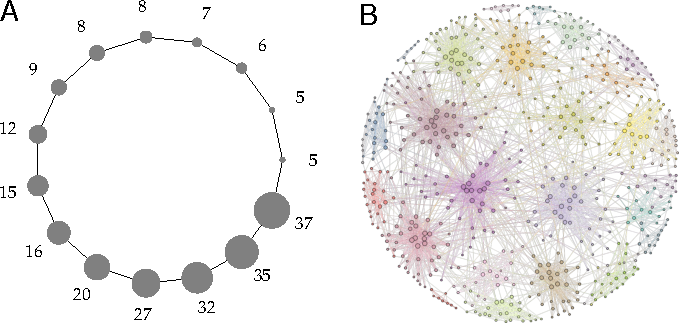
\includegraphics[width=1\textwidth]{images/pacopaperfigure1.pdf}
\caption{The two benchmark networks used in this study, laid out. (A) is a power-law ring of cliques, where cliques present different sizes sampled from a power-law distribution;
(B) is the layout of an LFR network with parameters $N=600$, $\left< k \right>=12$, $\max_k=50$, $\mu_t=0.1$, $\mu_w=0.1$, $\min_c=5$, $\max_c=50$.
The layout of (B) was generated with the graph-tool library~\cite{peixoto_graph_tool_2014}.}
\label{fig:lfrringclique}
\end{figure}

\begin{figure}[htb!]
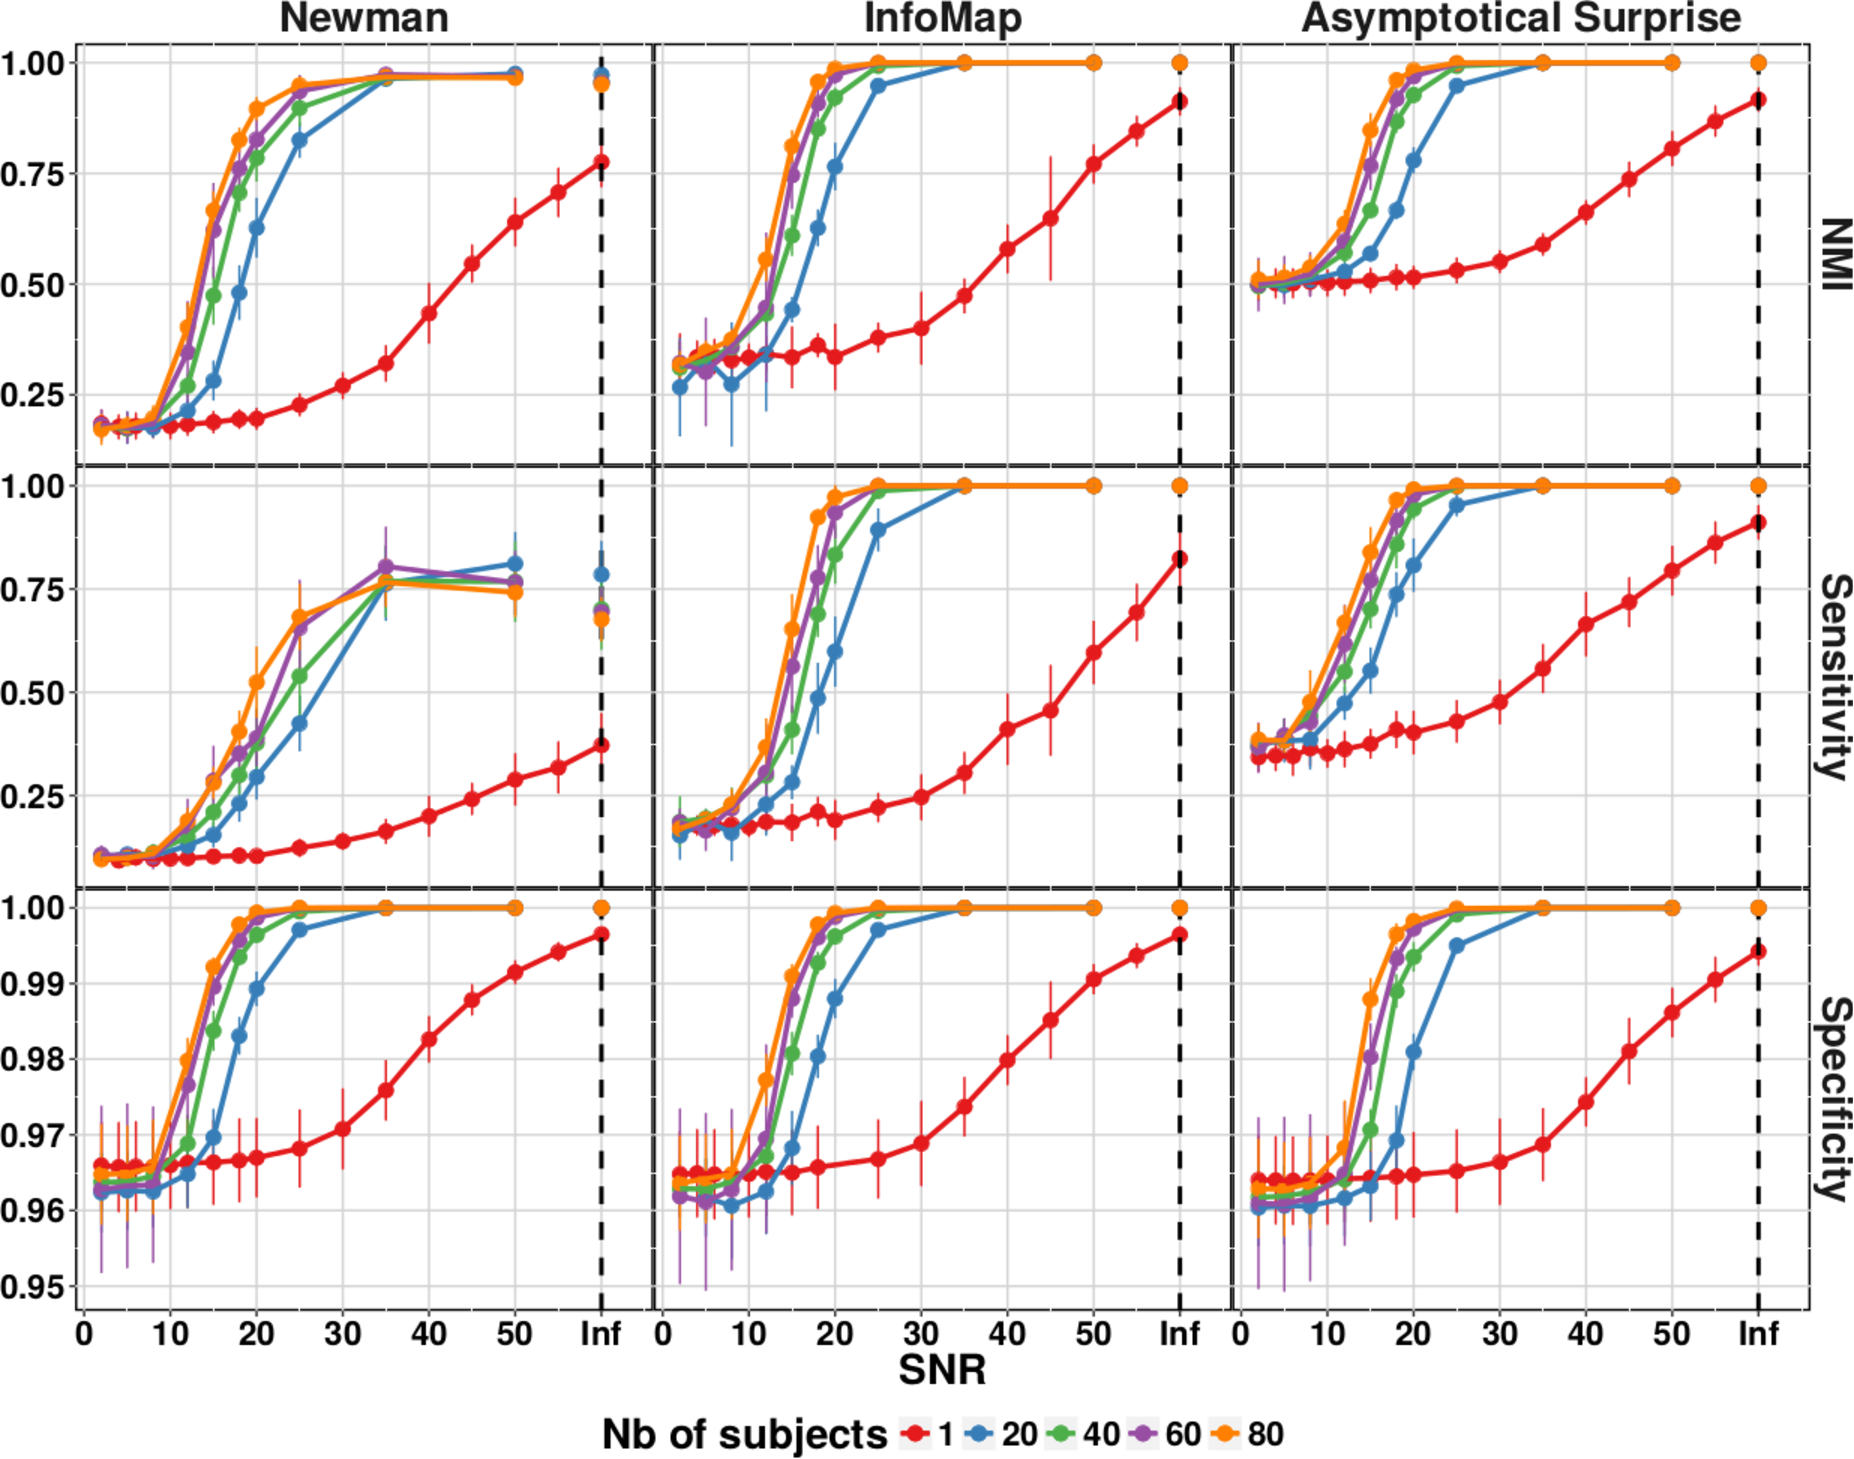
\includegraphics[width=\textwidth]{images/pacopaperfigure4.pdf}
\caption{NMI, Sensitivity and Specificity of the three community detection algorithms applied to a power-law ring of clique network. SNR indicates Signal to Noise Ratio, and Inf the situation with a network structure unperturbed by noise. Number of Subjects indicates the different number of instances used to generate the group level network.}
\label{fig:nmisensitivityspecificityringclique}
\end{figure}

Comparable results were obtained for the LFR network (Figure~\ref{fig:nmisensitivityspecificitylfr}), a model graph that replicates the distribution of nodal degree observed in many real-world networks, including those representing brain functional connectivity.
All three methods showed similar values of NMI for high SNR and a large number of subjects, with a plateau reaching maximum Sensitivity with a group sample bigger than $20$ and SNR above $30$.
Sensitivity was only slightly worse for Modularity, but it should be noted that for the LFR network the size distribution of the planted modules was narrower than for the ring of cliques (Figure~\ref{fig:lfrringclique}), thus making the resolution limit less evident.

\begin{figure}[htb!]
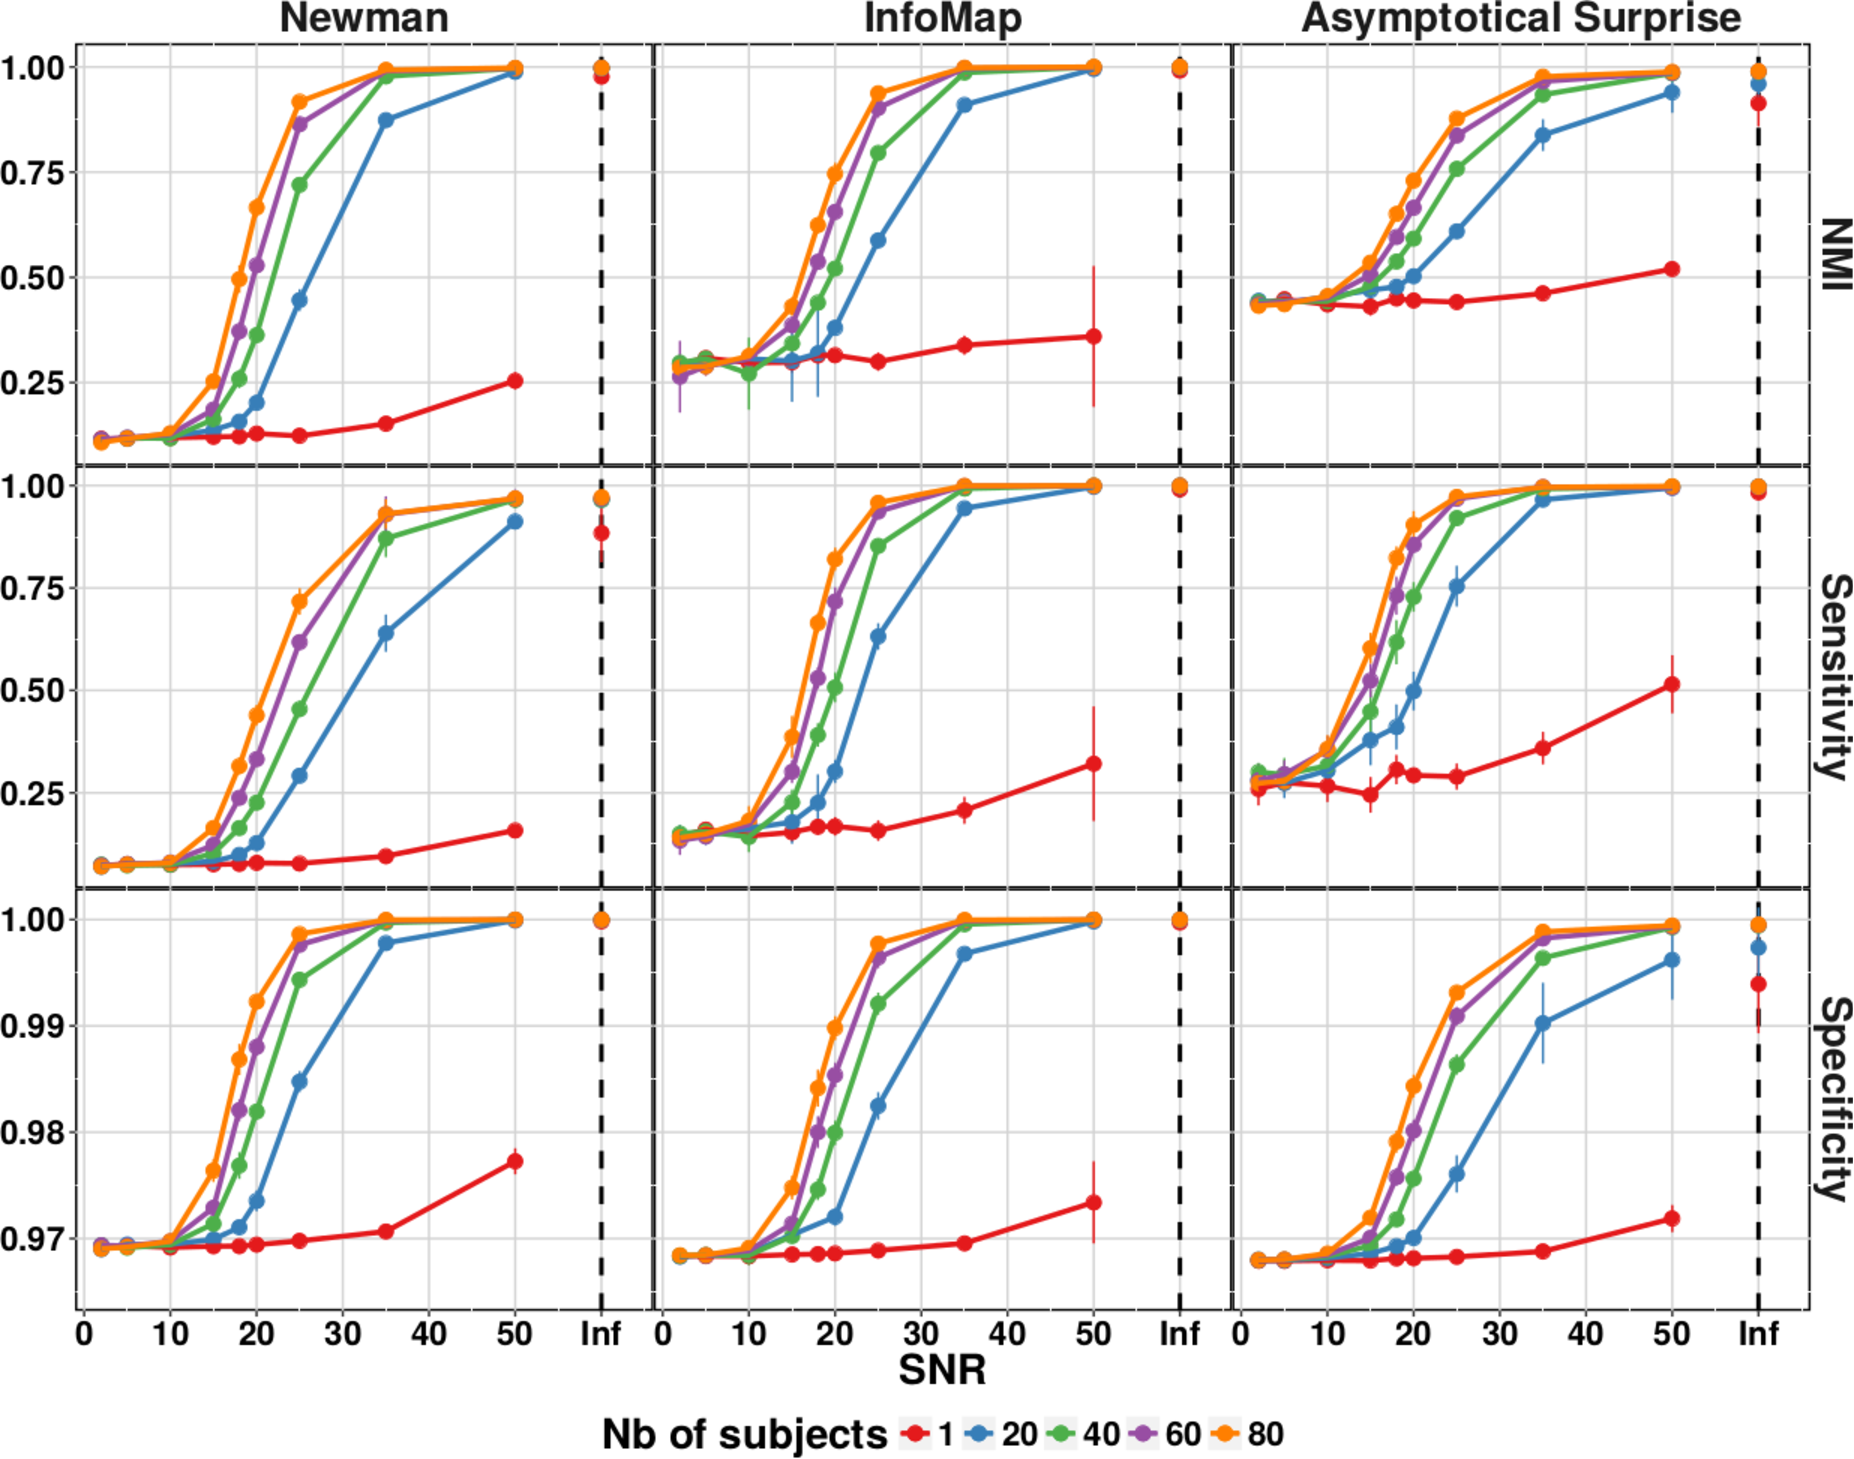
\includegraphics[width=\textwidth]{images/pacopaperfigure5.pdf}
\caption{NMI, Sensitivity and Specificity of the three community detection algorithms applied to Lancichinetti-Fortunato-Radicchi (LFR) networks. SNR indicates Signal to Noise Ratio, and Inf the situation with a network structure unperturbed by noise. Number of Subjects indicates the different number of instances used to generate the group level network.}
\label{fig:nmisensitivityspecificitylfr}
\end{figure}

In the lower SNR regime, Asymptotical Surprise presented the best performance in terms of NMI and Sensitivity, with a slower decay for decreasing SNR. 
Specificity was almost equivalent across the three methods, with a quick convergence to the maximum value of 1 for high SNR and good performance (around $0.97$) for low SNR.
Asymptotical Surprise presented a faster decay with decreasing SNR.
However, it should be noticed that the scale of Specificity has a very narrow range ($0.97$-$1.00$), and the differences between the three methods were relatively small.

Consensus analysis applied to Newman's Modularity to assess the potential effects of the degeneracy of nearly optimal solutions did not show substantial differences in the comparison with the other methods (Supplementary Information, Figure S6, S7).

For the sake of completeness, we also computed Accuracy and Matthew Correlation Coefficient for the same model networks, shown in the Supplementary Materials.
Notably, Infomap showed a large variability in Accuracy for lower SNRs and number of subjects.
Under closer examination, however, it appeared that the increased variance for Infomap was due to occasional runs in which the algorithm only retrieved one or two large modules.
This is a known problem with Infomap and other algorithms based on random walks that depends on the need to parametrize the teleportation step in order to make the dynamics ergodic~\cite{lambiotte2012}.

Altogether, the picture that emerges from the analysis of Accuracy and MCC is entirely consistent with the results shown in this section.

\subsection{Asymptotical Surprise on resting state dataset}
Figure~\ref{fig:partitioncomparison} shows a comparison between the modular structure of the resting state fMRI dataset obtained with Newman's Modularity, Infomap and Asymptotical Surprise.
For each method, we had $10,000$ independent runs and picked the partition with the best value of the respective fitness functions ($Q=0.4967$, $\mathcal{L}=8.5173$, $S_a=5925.3$, for Modularity, Infomap and Asymptotical Surprise, respectively).
The three methods showed significantly different partitions (relative NMIs in Table 1), with a number of detected communities of 10, 19 and 47 for Modularity, Infomap and Asymptotical Surprise, respectively.
Interestingly, Modularity detected a relatively uniform size distribution, consistent with the intrinsic scale built into the fitness function.
Infomap showed a wider distribution of module sizes, with number of nodes ranging between 156 and 3, while Surprise showed the largest spread, and included communities as small as single nodes (singletons).

\begin{figure}[htb!]
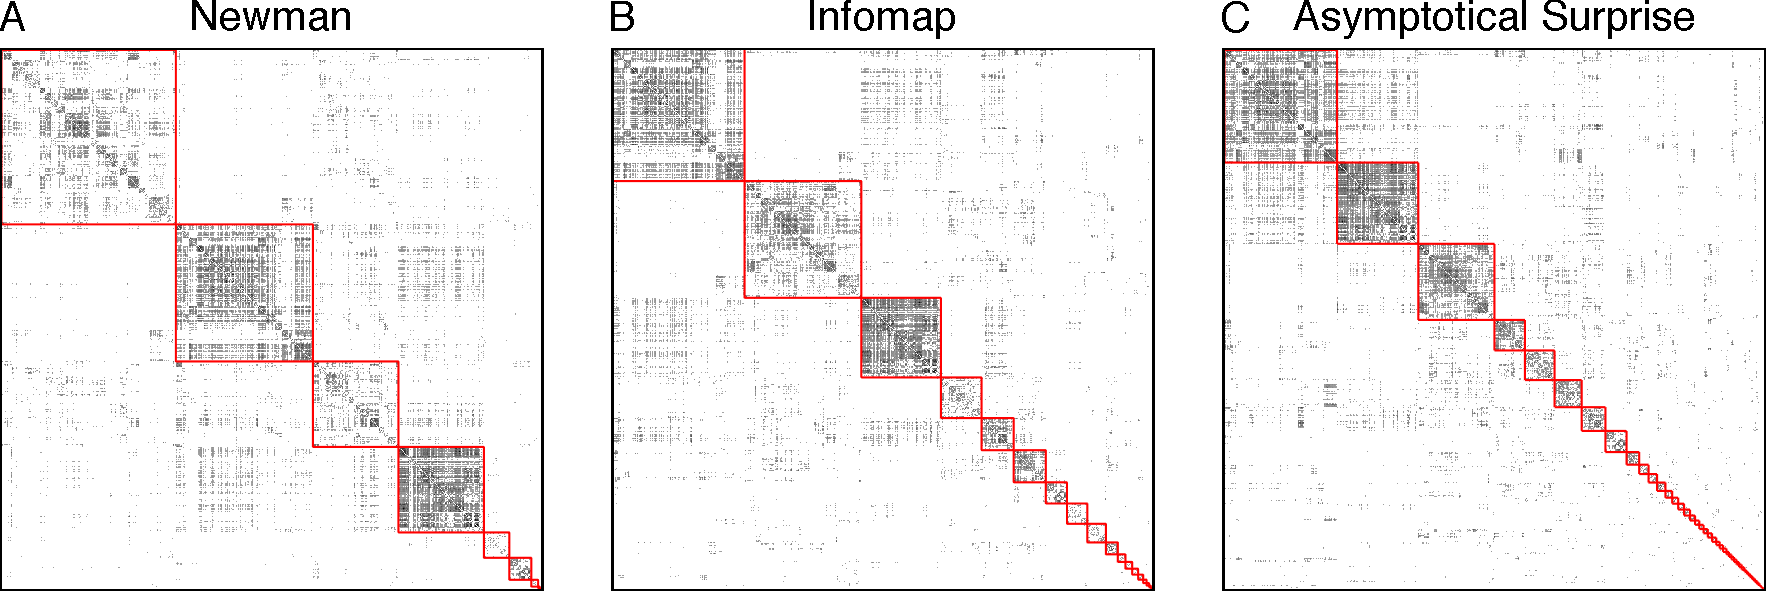
\includegraphics[width=\textwidth]{images/pacopaperfigure6.pdf}
\caption{Adjacency matrix of the resting state functional connectivity network. The node indices have been reordered by module membership in each graph, and the red lines highlight the community structures obtained by A) Louvain-Newman's Modularity ($Q=0.4967$); B) Infomap ($L=8.5173$); C) Asymptotical Surprise ($S_a=5925.28$).}
\label{fig:partitioncomparison}
\end{figure}


Figure~\ref{fig:cervellini4x4} shows the 16 largest modules detected by Asymptotical Surprise, ranked by number of nodes comprised in each community. 
The first and largest module (Fig. \ref{fig:cervellini4x4}A) includes the pre- and post-central gyri, part of the supramarginal gyrus and supplementary motor area.
The second community (Fig. \ref{fig:cervellini4x4}B) consists largely of nodes belonging to the occipital lobe: the visual areas and the surrounding calcarine sulcus, the lingual and fusiform gyrus.
The third module (Fig. \ref{fig:cervellini4x4}C) reflects the Default Mode Network, spanning the temporo-parietal cortex, the medial prefrontal cortex and the posterior cingulate/precuneus.
The nodes involved in the executive frontal functions form the fourth largest community.
Interestingly, nodes in the communities D, E, G are the major players that take part in the so-called fronto parietal attentional network~\cite{markett2014}.
The auditory network, comprising temporal areas, was detected as a distinct community (Fig. \ref{fig:cervellini4x4}F).
Deeper structures emerge as separate modules in Fig. \ref{fig:cervellini4x4}H, with subcortical areas including the basal ganglia, i.e. putamen, globum pallidum, caudate nucleus and the whole thalamus.
The hippocampus and the parahippocampal gyrus were identified as separate communities (O and P).
Additional, smaller substructures are shown in the third and fourth row of Figure~\ref{fig:cervellini4x4}, including the Supplementary Motor Area (Fig. \ref{fig:cervellini4x4}J) and the orbital (Fig. \ref{fig:cervellini4x4}M) and orbitofrontal (Fig. \ref{fig:cervellini4x4}I) modules, containing nodes from Brodmann area 47 (the smaller communities are displayed Figure S8).

\begin{figure}[htb!]
\includegraphics[width=\textwidth]{images/pacopaperfigure7.pdf}
\caption{Sixteen largest modules found by Asymptotical Surprise Maximization in the resting state network overlaid on an MRI brain template. The modules are ranked by decreasing size, and named after corresponding functional networks previously identified by multivariate analysis of resting state fMRI data, or by the comprised anatomical districts.}
\label{fig:cervellini4x4}
\end{figure}

Partitions of the functional connectivity network obtained by Newman's Modularity and Infomap are reported in the Supplementary Materials Section (Figures S9 and S10).
Newman's Modularity retrieved four large, relatively uniform communities, corresponding to the Default Mode Network, the central network, occipital and frontoparietal networks.
This is in keeping with previous studies using Modularity optimization by spectral decomposition~\cite{crossley2013a}, and consistent with the strong resolution limit that affects this method.
Additionally, a few smaller modules were found by Louvain optimization of Newman's Modularity, corresponding to the basal ganglia, the hippocampal/parahippocampal formation and two asymmetrically distributed subcortical clusters.

Infomap identified 19 communities of various sizes, also shown in the Supplementary Materials Section, Figure S10.
The largest modules showed a close correspondence with those identified by Asymptotical Surprise, albeit with some notable differences.
By way of example, the largest component includes the motor-sensory and auditory modules, identified as separate communities by Asymptotical Surprise.
The Default Mode Network retrieved by Infomap includes parts of the temporal cortices that are not normally associated with the DMN.
Similarly, hippocampus and the parahippocampal modules were merged by Infomap, and resolved as individual modules by Asymptotical Surprise.
Other modules, including the visual, associative and executive networks (C, E and F in Figure S10, respectively) were qualitatively very similar to those identified by Asymptotical Surprise.

Altogether, the picture that emerges is consistent with the idea that the resolution limit is more severe in Newman's Modularity than in Infomap, and that Asymptotical Surprise presents the best resolving power among the three methods in a real-world network with finite SNR and variability as the resting state functional connectivity network used for this study.

\subsection{Hub classification}
Maps of the anatomical distribution of the participation coefficient and within module degree show substantial differences between the three community detection methods (Figure~\ref{fig:hubclassification}), resulting in discrepancies in the identification of the connector hubs for the same functional connectivity network.

Figure~\ref{fig:hubclassification_threshold} shows the nodes with simultaneously high values of participation coefficient and within module degree (connector hubs, according to the Guimera and Amaral's classification).
All three methods pinpoint connector hubs in the superior, superior medial and middle frontal areas, as well as in the supplementary motor area.
However, substantial differences are observed for other hub regions. The partition of Asymptotical Surprise localizes connector hubs in the Temporal Middle and Frontal Middle gyri, as well as in the Rectus, Middle Cingulate Cortex, Lingual gyrus and in the Precuneus.

Community detection by InfoMap results in the identification of hubs that are partially consistent with either of the two other methods, in keeping with the idea that its resolution limit is less severe than for Newman's Modularity.
Altogether, these findings indicate that node role classification is method-dependent, and may be affected by the resolution limit.

\begin{figure}[htb!]
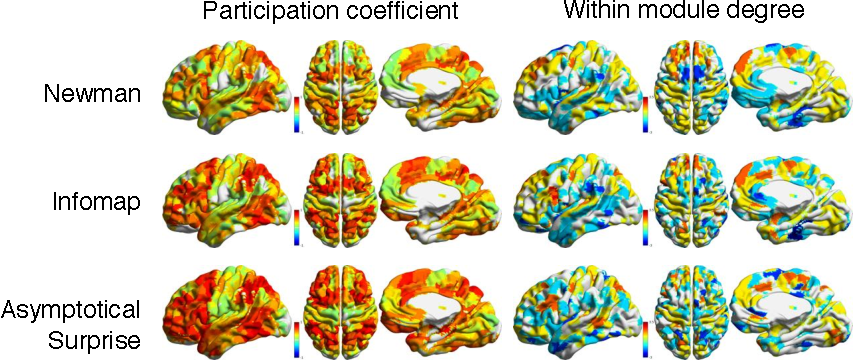
\includegraphics[width=\textwidth]{images/pacopaperfigure8.pdf}
\caption{Anatomical distributions of the participation coefficient and within-module degree z-score for the resting state functional connectivity network partitioned by the three community detection methods.}
\label{fig:hubclassification}
\end{figure}


\begin{figure}[htb!]
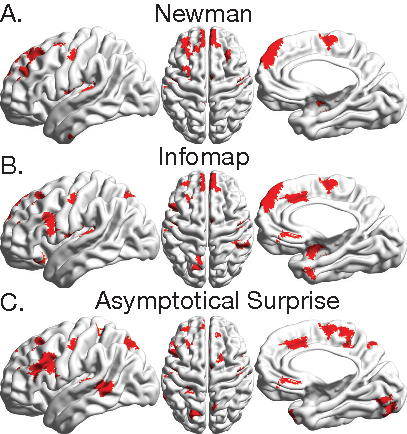
\includegraphics[width=\textwidth]{images/pacopaperfigure9.pdf}
\caption{Nodes presenting simultaneously large values of the participation coefficient and within-module degree (larger than 0.6 and 1.5, respectively) for the three community detection methods. These nodes are thought to represent the connector hubs responsible for the integration of the networks's modules.
}
\label{fig:hubclassification_threshold}
\end{figure}

\subsection{Validation of Asymptotical Surprise in model networks}
The performance of Asymptotical Surprise optimization by PACO was assessed in model graphs with a built-in community structure, and compared with two established community detection methods. We have chosen two synthetic benchmark networks, the ring of cliques and the LFR network.

The ring of cliques presents a clear-cut modular structure by construct, with modules corresponding to complete subgraphs of variable sizes sampled from a power-law distribution. 
This toy network proved useful to assess the effects of the resolution limit in the presence of a wide distribution of cluster sizes. The effects of this limit were particularly apparent for Newman's Modularity (Figure~\ref{fig:nmisensitivityspecificityringclique}), that showed poor Sensitivity even for noiseless rings of cliques, plateauing at a value of $0.75$.
This is consistent with the findings of~\cite{fortunato2007}, that showed that for Modularity the resolution limit is set by the square root of the total number of edges in the graph.
For Infomap, this limit is less severe and is determined by the number of inter-cluster edges~\cite{kawamoto2015}. Accordingly, the effects of the resolution limit were not apparent in this model network, where modules are sparingly connected by single edges.
Asymptotical Surprise presented the best performance, consistent with the idea that this cost function is quasi-resolution limit free~\cite{traag2015}.

However, real brain networks are characterized by heterogeneous distributions of node degree, with fat tails and power-law decays~\cite{bullmore2009}. Such heterogeneity is critical, as it determines some of the remarkable features of brain connectivity networks, including resilience to random failure and rich-clubness~\cite{vandenheuvel2011,vandenheuvel2013a}. To provide a more realistic benchmark, we used the Lancichinetti-Fortunato-Radicchi algorithm~\cite{lancichinetti2008}, that makes it possible to generate networks with realistic and tunable power law degree distribution and community sizes.

For LFR networks, the difference in performance in the low-noise regime was more nuanced for the three methods compared in this study, possibly a result of a fuzzier community structure of the LFR network compared to the ring of cliques, and of the narrower distribution of cluster sizes. However, the picture appears different when noise and intersubject variability were injected into the network structure.

Noise and other sources of variability in the data can significantly affect the structure of the resulting network representation.
Noisy fMRI time-courses, for example, may introduce spurious correlations in brain functional connectivity networks.
This problem may be particularly relevant for methods endowed with high resolution, like Asymptotical Surprise, that may be more vulnerable to False Positives generated by the mis-assignment of peripheral nodes, particularly in small clusters. Hence, the resolving power of community detection methods should be gauged against Specificity, which may be affected by noise in the distribution of edges that define the network's structure.
However, to the best of our knowledge, this aspect has never been considered in the existing literature assessing the performance of community detection algorithms as applied to the study of brain connectivity.

To this end, we have devised methods to inject noise, with amplitude and spectral distribution that mimic those of experimental noise, into networks with a well defined planted structure. Moreover, we have generated different instances for each network, corresponding to different subjects in a group, to account for intersubject variability that occurs in typical neuroimaging studies. 

Unsurprisingly, for all methods and networks, detection of the planted structure improved with decreasing levels of noise, and with increasing number of subjects in the study.
However, Asymptotical Surprise appeared to provide a superior performance in terms of NMI and Sensitivity to the planted structure for lower SNRs in both types of networks, while its Specificity was in line with that of resolution-limited methods like Newman's and Infomap (Figures \ref{fig:nmisensitivityspecificityringclique},\ref{fig:nmisensitivityspecificitylfr}).
This rules out the idea that the higher sensitivity to small clusters of Asymptotical Surprise may be detrimental in noisy networks, making it more vulnerable to small, spurious modules.

\subsection{Asymptotical Surprise optimization on resting state networks}
Application of Asymptotical Surprise maximization to a group-level, resting state functional connectivity network from the brains of $27$ healthy subjects revealed a heterogeneous distribution of modules, with large and small modules coexisting in the optimal partition.
This is in keeping with previous findings with binary Surprise~\cite{nicolini2016}.
These modules closely reflect functional networks reported in many studies using Independent Component Analysis or other multivariate methods, including the sensorimotor, visual, default mode, executive, and attentional networks.
Moreover, anatomically defined subcortical structures, like the hippocampus and parahippocampal formations emerged as independent moduli.

While this is entirely consistent with our understanding of the neurofunctional and anatomical organization of the human brain, the accuracy of Asymptotical Surprise in identifying these networks is notable.
Indeed, Surprise, like other graph-based community detection methods, divides networks into disjoint clusters of nodes on the basis of topological criteria.
While a correspondence between topological modularity and functional networks identified by, e.g. Independent Component Analysis, may be expected, it is not a given, for they are defined on different principles. Indeed, multivariate methods like ICA separate components on the basis of the statistical independence of the time-courses, and do not convey information regarding the mutual relationship between modules nor about their topological organization.

Previous studies applying resolution-limited methods like Newman's Modularity to the same dataset hereby analyzed~\cite{crossley2013a} found a few, large modules encompassing large-scale networks, but failed to identify finer, neurofunctionally plausible substructures like those shown in the present study. Infomap, on the other hand, proved sensitive to heterogeneously distributed clusters, thus implying that this method does not have an intrinsic scale, like Modularity and variations thereof based on the introduction of a resolution parameter. 
However, Asymptotical Surprise appears to provide superior performance in identifying small subnetworks, particularly in the presence of noise, thus suggesting that this method may represent a new standard for community detection in brain networks. It should also be noted that no symmetry constraint was imposed, and the symmetrical bilateral distribution of nodes in the retrieved modules arises entirely from Asymptotical Surprise optimization. 

Hierarchical clustering methods have been extensively applied to investigate the structure of brain connectivity networks, showing smaller and smaller clusters as the modules are iteratively subdivided~\cite{meunier2010}. Maximization of Asymptotical Surprise reflects the optimal cut through the dendrogram representing connectivity at these different levels of subdivision, and provides information on the optimal partition of the network. Hence, the heterogeneous distribution of cluster sizes retrieved by Asymptotical Surprise suggests that multiple scales of structure exist at the same level of the dendrogram.

Finally, abnormal functional connectivity has been observed in a number of neurological and psychiatric diseases, but the coarse resolution of methods like Newman's Modularity~\cite{fornito2015} may have not detected differences in the modular organization of networks in patients compared to healthy controls. The improved resolution and sensitivity to multiscale structure afforded by Asymptotical Surprise may provide a powerful means to assess the brain functional architecture in disease states, thus contributing a potential imaging-based marker and a key to interpret the functional effects of aberrant connectivity.
\subsection{Hub classification}
The presence of heterogeneously distributed modules in functional connectivity networks may have important consequences for our understanding of the brain functional organization. By way of example, it has been shown that highly connected nodes, or hubs, are critically important in brain connectivity networks, and may play different roles depending on their position and connectivity distribution within and between modules~\cite{bullmore2009}. Hubs that primarily connect to nodes within the same community are dubbed “provincial hubs”, and are thought to be responsible for the definition and stability of the modules. Conversely, hubs that connect different modules are referred to as “connector hubs” and ensure integration of the activity of the network. The classification of hubs strongly depends on the modular structure that is considered, and inaccurate partitioning due to the resolution limit can lead to the wrong interpretation of their role in the interplay between segregation and integration of brain function~\cite{bullmore2009}. The present study suggests that this may have been the case in previous studies, in which resolution limited methods characterized by an intrinsic scale have been used, and provides a solution that may enable more accurate classification of hubs and nodes.

The connector hubs identified by our three methods (Asymptotical Surprise, InfoMap and Newman) present some substantial differences, consistent with the idea that hub classification depends on community structure. These differences are particularly interesting in the light of the important role that connector hubs are thought to play in integrating information flow through the brain, and their putative role in brain disease \cite{crossley2014,stam2014}. By way of example, the Precuneus and the Cingulate Cortex are highlighted by Asymptotical Surprise, but not by Newman's Modularity, as connector hubs. These are two key elements of the Default Mode Network that have been consistently identified as vulnerable regions in neurological diseases~\cite{vandenheuvel2013a,buckner2009}. 
Community detection by resolution limited free methods should enable more accurate classification of hub nodes, and improve our understanding of their role in brain disease. 

\subsection{Limitations of Asymptotical Surprise}
Some caution should be taken in the interpretation of the graphs in Figures \ref{fig:nmisensitivityspecificityringclique} and \ref{fig:nmisensitivityspecificitylfr}.
Indeed, the SNRs of the synthetic networks we have generated reflect noise with features, like a Rician distribution, that mimic some, but not all aspects of the variability of experimental data.
By way of example, the brain parcellation scheme applied to define the nodes, and the heterogeneity of voxels within these parcels, may play a role that is difficult to model in toy networks~\cite{fornito2010}.
Hence, the simulated Sensitivity and Specificity as a function of SNR and number of subjects should not be taken as absolute values to be used in the power and sample size estimation in real experimental designs.
Nevertheless, these simulations provide useful information on the dependence of these parameters on noise levels, and a rigorous means to assess the relative merits of different community detection methods.

Finally, we should note that the maximum value of Asymptotical Surprise calculated with PACO is an index of quality of the entire partition, and not of individual modules.
Hence, individual modules may not all have the same strength of internal cohesiveness relative to their connection with other modules.
We have found hints of this phenomenon in the comparison of nearly-optimal partitions obtained in the $10,000$ runs of PACO that we have performed to find the optimal community structure for this network.
The overall community structure appeared to be robust, with most modules persistently emerging in every nearly-optimal partition, but in some cases we observed pairs of modules splitting or merging in otherwise similar solutions. Most notably, this was observed for the thalamus that in some instances was merged with the basal cluster and in others, featured as a separate module.
This phenomenon may be less critical for methods like Newman's Modularity that have an intrinsic scale and retrieve uniformly distributed modules.

\section{Conclusions}
We have extended the use of Surprise, a resolution-limit-free fitness function for the study of the modular structure of complex networks, to weighted brain functional connectivity networks. Specifically, we have developed a novel method, dubbed PACO, for the optimization of Asymptotical Surprise, a weighted counterpart of Surprise in the limit of large networks. We have applied PACO optimization of Asymptotical Surprise in synthetic networks to evaluate the relative merits of this novel approach against Newman's Modularity and Infomap, two of the leading methods used for community detection in brain connectivity networks. Specifically, we have implemented a process to inject noise into networks endowed with a ground-truth modular structure to assess the trade-off between improved resolution afforded by Asymptotical Surprise and potential sensitivity to spurious correlations introduced by variability in the data. Asymptotical Surprise optimization proved superior to existing methods in terms of Sensitivity and accuracy in detection of the planted structure as measured by Normalized Mutual Information, while showing comparable Specificity. We have also applied our approach to the partitioning of functional connectivity networks from resting state fMRI experiments. Direct comparison with other methods clearly demonstrated improved capability to identify neurofunctionally plausible and anatomically well-defined substructures otherwise concealed by the resolution limit. Asymptotical Surprise revealed a complex modular structure of resting state connectivity, with communities of widely different sizes reflecting distributed functional networks alongside with small, anatomically or functionally defined modules. This evidence corroborates the idea that the resolution limit may have negatively affected current models of the brain modular organization and the identification of the hubs responsible for integration of functional modules. 
The application of methods like Asymptotical Surprise provides a novel, powerful approach to study the modular structure of brain connectivity beyond this limit.
